\documentclass[12pt,a4paper]{article}
\usepackage[utf8]{inputenc}
\usepackage[T1]{fontenc}
\usepackage[polish]{babel}
\usepackage{graphicx}
\usepackage{geometry}
\usepackage{amsmath}
\usepackage{booktabs}
\usepackage{caption}
\usepackage{subcaption}
\usepackage{float}
\usepackage{hyperref}
\usepackage{siunitx}
\usepackage{indentfirst}
\usepackage{parskip}

\geometry{
    a4paper,
    left=2.5cm,
    right=2.5cm,
    top=2.5cm,
    bottom=2.5cm
}

\hypersetup{
    colorlinks=true,
    linkcolor=black,
    urlcolor=black
}

\begin{document}

%% ============================================================
%% STRONA TYTUŁOWA
%% ============================================================
\begin{titlepage}
    \centering
    \vspace*{\fill}
    \begin{figure}[h]
        \centering
        
\includegraphics[width=0.95\textwidth]{images/pwr_logo.png}
    \end{figure}
    \vspace{0.75cm}
    {\huge\bfseries RAPORT Z PROJEKTU\par}
    \vspace{0.75cm}
    {\Large\bfseries Temat:\par}
    {\huge\bfseries Projekt i symulacja synchronicznej przetwornicy buck z sterowaniem PWM via ESP8266\par}
    \vspace{0.75cm}
    {\Large\bfseries Autor:\par}
    {\large Piotr Rosiński\par}
    \vspace{0.75cm}
    {\large Wydział Elektroniki, Fotoniki i Mikrosystemów\par}
    {\large Kierunek: Elektronika\par}
    {\large Specjalność: Aparatura elektroniczna\par}
    {\large Promotor: dr inż. Mateusz Bartczak\par}
    \vspace{1cm}
    {\large Miejsce i rok: Wrocław, 2025\par}
    \vspace*{\fill}
\end{titlepage}

%% ============================================================
%% SPIS TREŚCI
%% ============================================================
\tableofcontents
\newpage

%% ============================================================
%% 1. WSTĘP TEORETYCZNY
%% ============================================================
\section{Wstęp teoretyczny}

\subsection{Przetwornica buck}

Przetwornica buck (przetwornica obniżająca napięcie) jest topologią przekształtnika DC/DC
pracującego w trybie impulsowym (ang. \textit{Switched Mode Power Supply}, SMPS).
Podstawowa zasada działania polega na naprzemiennym włączaniu i wyłączaniu tranzystora
mocy z częstotliwością $f_{sw}$, co pozwala na regulację napięcia wyjściowego $V_{out}$
zgodnie z zależnością:

\begin{equation}
    V_{out} = D \cdot V_{in}
    \label{eq:buck_basic}
\end{equation}

\noindent gdzie $D \in \langle 0, 1 \rangle$ oznacza współczynnik wypełnienia sygnału PWM
(ang. \textit{Duty Cycle}), $V_{in}$ -- napięcie wejściowe.

\subsection{Topologia synchroniczna}

W klasycznej przetwornicy buck dioda swobodna jest zastępowana tranzystorem
mocy sterowanym komplementarnie do tranzystora głównego (rys.~\ref{fig:ltspice_sch}).
Topologia synchroniczna charakteryzuje się:

\begin{itemize}
    \item mniejszymi stratami przewodzenia (napięcie nasycenia MOSFET $V_{DS(on)} \ll V_F$ diody),
    \item wyższą sprawnością przy dużych prądach obciążenia,
    \item koniecznością zastosowania układu \textit{dead time} zapobiegającego
          zwarciu (\textit{shoot-through}).
\end{itemize}

\subsection{Dead time}

W półmostku z tranzystorami Q1 (high-side) i Q2 (low-side) jednoczesne
przewodzenie obu tranzystorów powoduje zwarcie napięcia wejściowego do masy.
Zjawisko to nosi nazwę \textit{shoot-through}. Sterownik IR2112 generuje sprzętowo
\textit{dead time} wynoszący $t_{DT} \approx \SI{520}{ns}$, podczas którego oba
tranzystory pozostają wyłączone.

\subsection{Tryby pracy cewki}

W zależności od wartości indukcyjności, częstotliwości przełączania i prądu obciążenia
przetwornica może pracować w dwóch trybach:

\begin{itemize}
    \item \textbf{CCM} (ang. \textit{Continuous Conduction Mode}) -- prąd cewki
          nie spada do zera,
    \item \textbf{DCM} (ang. \textit{Discontinuous Conduction Mode}) -- prąd cewki
          spada do zera przed kolejnym cyklem przełączania.
\end{itemize}

Graniczna indukcyjność dla trybu CCM wyraża się wzorem:

\begin{equation}
    L_{min} = \frac{(1-D) \cdot R_{load}}{2 f_{sw}}
    \label{eq:lmin}
\end{equation}

\subsection{Zjawisko EMI}

Strome zbocza napięcia w węźle przełączającym $V_{SW}$ są głównym źródłem
zakłóceń elektromagnetycznych (ang. \textit{Electromagnetic Interference}, EMI).
Przy częstotliwościach przełączania \SIrange{200}{300}{kHz} harmoniczne sygnału
obejmują szerokie widmo, interferując z innymi urządzeniami elektronicznymi.

%% ============================================================
%% 2. OPIS UKŁADU
%% ============================================================
\section{Opis zaprojektowanego układu}

\subsection{Schemat ideowy}

Zaprojektowany układ (rys.~\ref{fig:ltspice_sch}) jest synchroniczną przetwornicą buck
opartą na następujących komponentach:

\begin{table}[H]
    \centering
    \caption{Wykaz głównych komponentów układu}
    \label{tab:bom}
    \begin{tabular}{lll}
        \toprule
        \textbf{Oznaczenie} & \textbf{Komponent} & \textbf{Funkcja} \\
        \midrule
        Q1 (M1) & IRFP4668 / IRFS4x & Tranzystor high-side \\
        Q2 (M2) & IRFP4668 / IRFS4x & Tranzystor low-side \\
        IC1     & IR2112             & Sterownik bramek z bootstrap \\
        L1      & \SI{100}{\micro H} & Cewka filtrująca \\
        C1      & \SI{100}{\micro F} & Kondensator wyjściowy \\
        C2      & \SI{100}{\micro F} & Kondensator wyjściowy \\
        D1, D2  & 1N4148             & Diody ochronne bramek \\
        R1--R4  & rezystory bramkowe & Ograniczenie $\frac{dI}{dt}$ \\
        NodeMCU & ESP8266            & Generator PWM \\
        \bottomrule
    \end{tabular}
\end{table}

\noindent Parametry nominalne układu:
\begin{itemize}
    \item Napięcie wejściowe: $V_{in} = \SIrange{24}{100}{V}$ DC
    \item Napięcie wyjściowe: regulowane przez $D$
    \item Częstotliwość przełączania: $f_{sw} = \SI{50}{kHz}$
\end{itemize}

\begin{figure}[H]
    \centering
    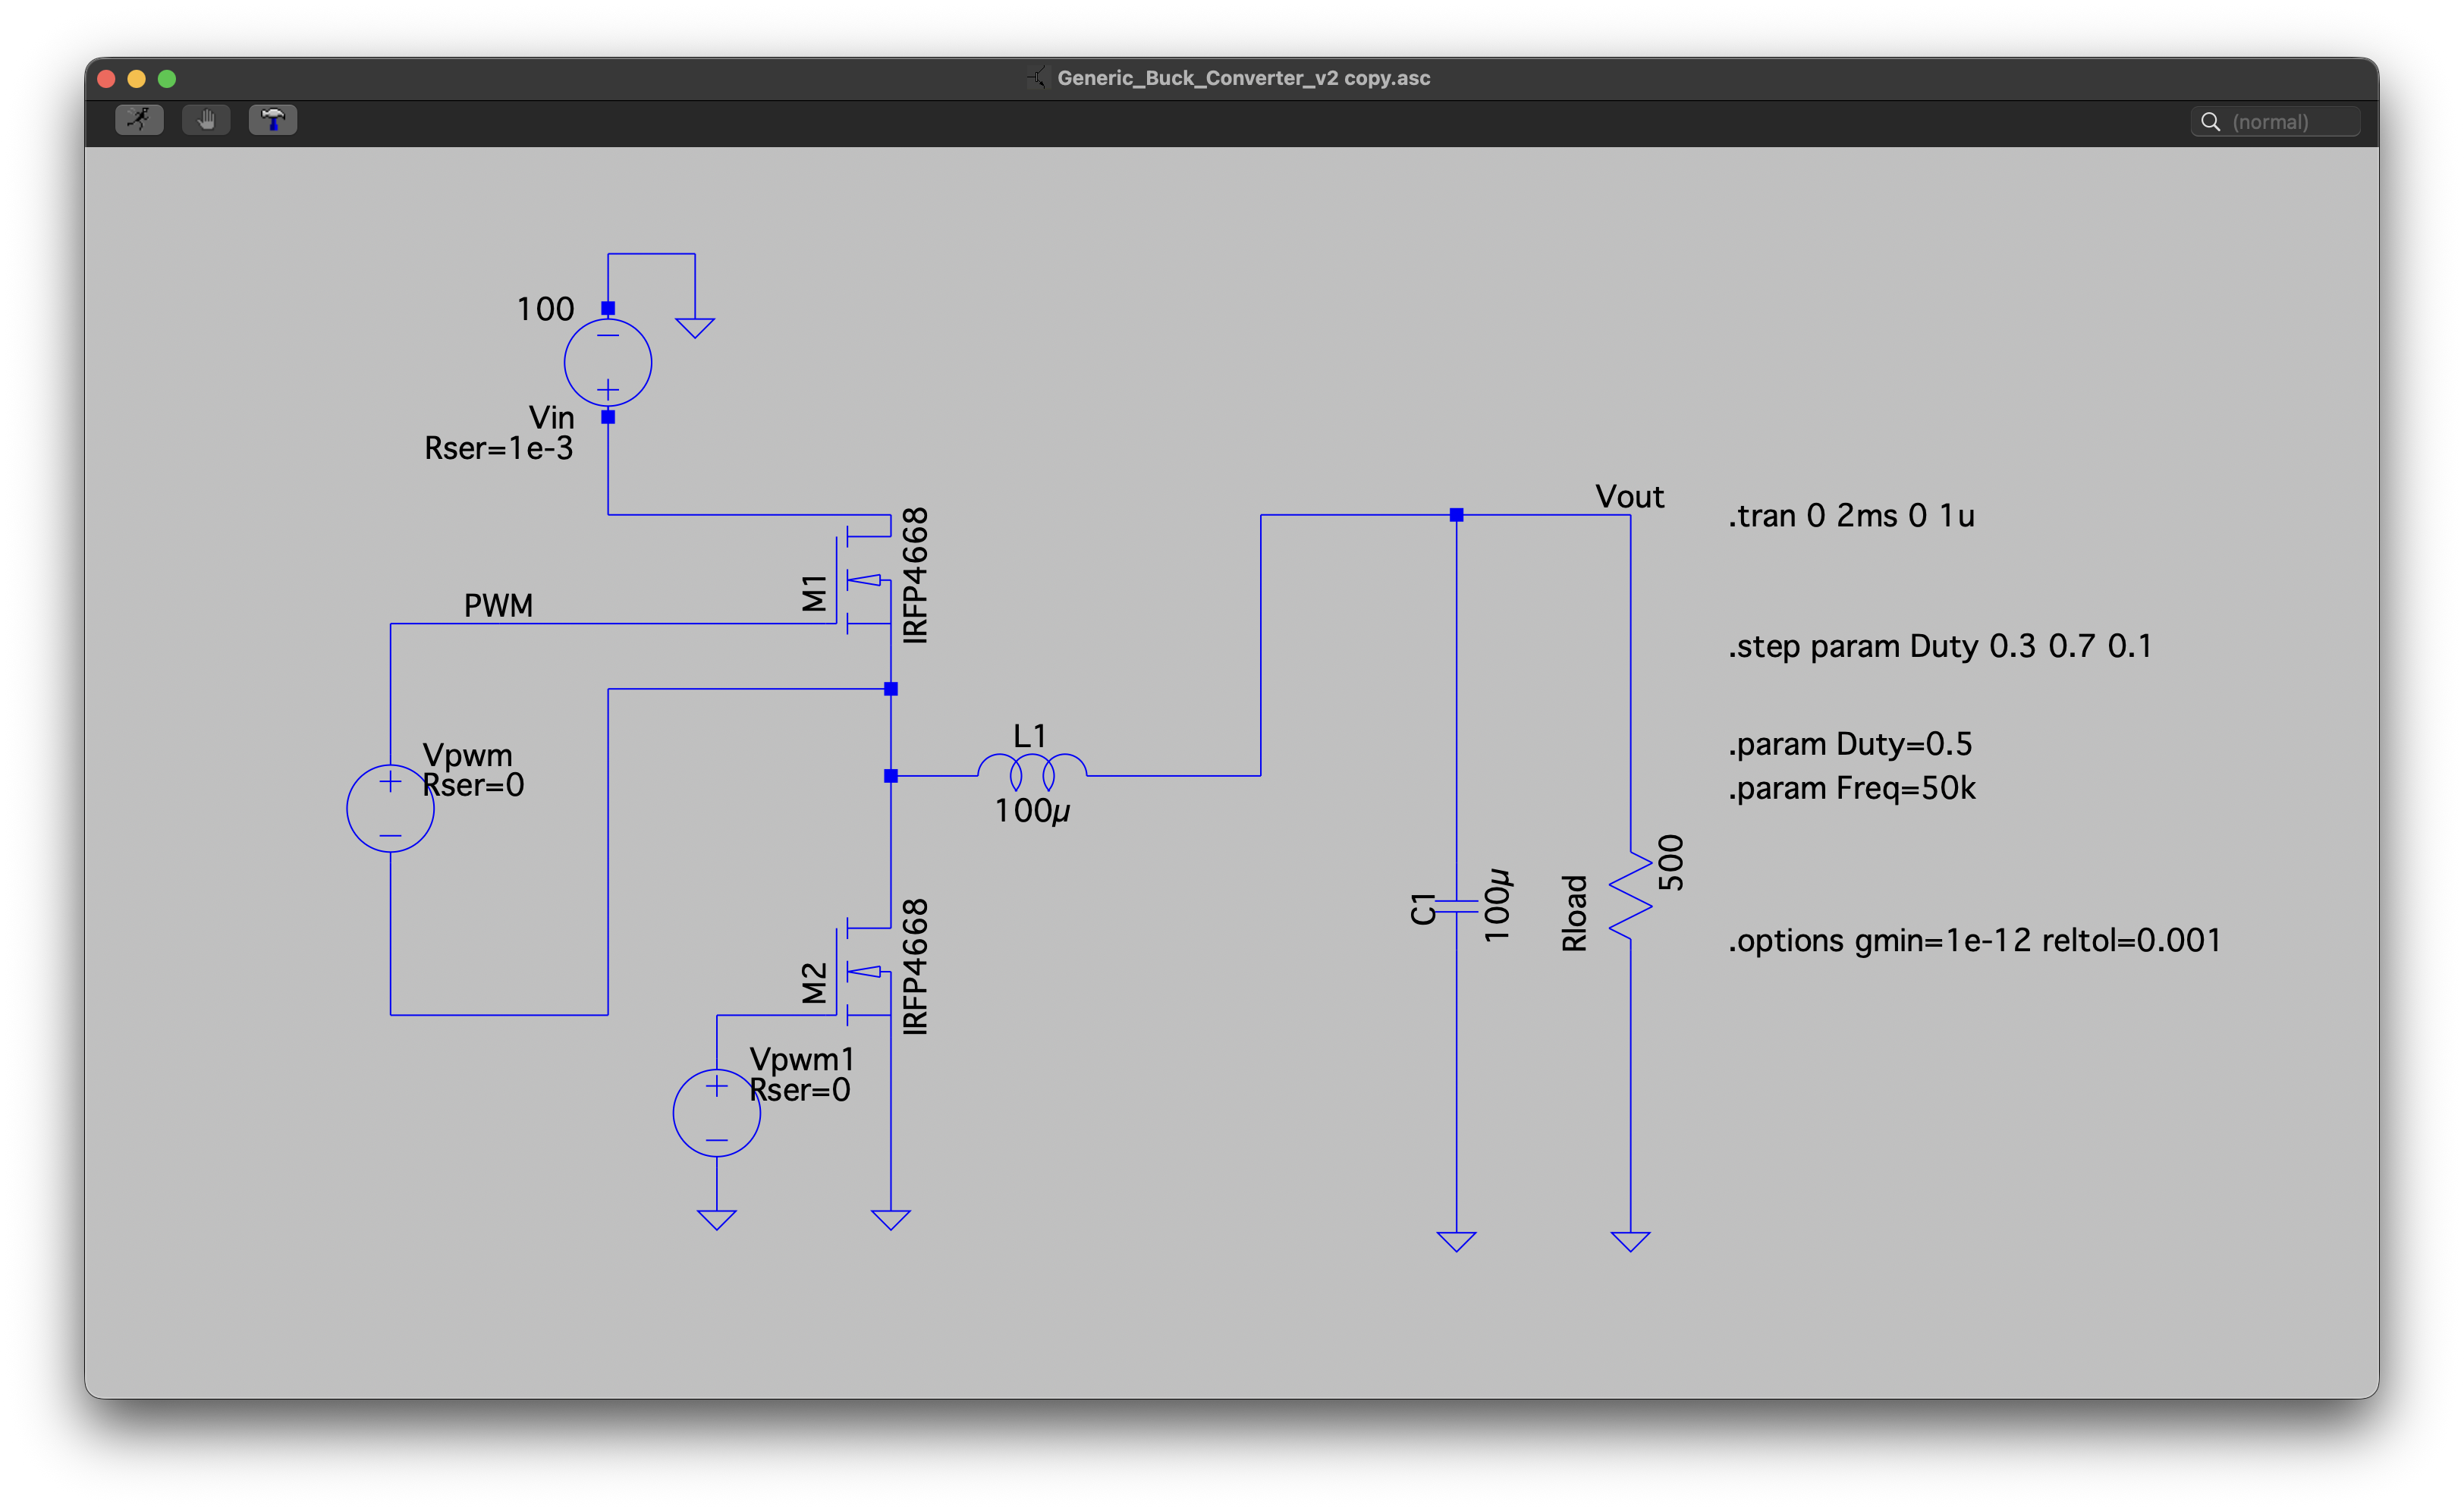
\includegraphics[width=0.9\textwidth]{LTSpice_layout.png}
    \caption{Schemat symulacyjny przetwornicy buck w LTSpice}
    \label{fig:ltspice_sch}
\end{figure}

\subsection{Sterownik IR2112 i układ bootstrap}

Sterownik IR2112 umożliwia sterowanie tranzystorem high-side pływającym na potencjale
węzła $V_{SW}$. Napięcie bramki Q1 jest generowane przez kondensator bootstrap $C_3$,
ładowany podczas przewodzenia Q2. W symulacji LTSpice układ bootstrap zastąpiono
izolowanym źródłem napięcia $V_{pwm}$, którego biegun ujemny podłączono do węzła SW.

\subsection{Sterownik PWM -- ESP8266 (NodeMCU V2)}

Mikrokontroler ESP8266 na module NodeMCU V2 generuje sygnał PWM o regulowanym
wypełnieniu $D$, przekazywany do wejścia HIN sterownika IR2112. Moduł umożliwia
zdalne sterowanie przetwornicą przez Wi-Fi, co czyni układ elementem systemu IoT.
Wbudowana antena IFA pracująca w paśmie ISM 2,4~GHz zapewnia łączność bezprzewodową.

%% ============================================================
%% 3. PROJEKT PCB
%% ============================================================
\section{Projekt płytki PCB}

Projekt płytki drukowanej wykonano w programie Autodesk EAGLE 9.6.2.
Płytka dwuwarstwowa (FR4, \SI{1.6}{mm}) zawiera wszystkie komponenty wykazu BOM
(tab.~\ref{tab:bom}).

\begin{figure}[H]
    \centering
    \begin{subfigure}[b]{0.48\textwidth}
        \centering
        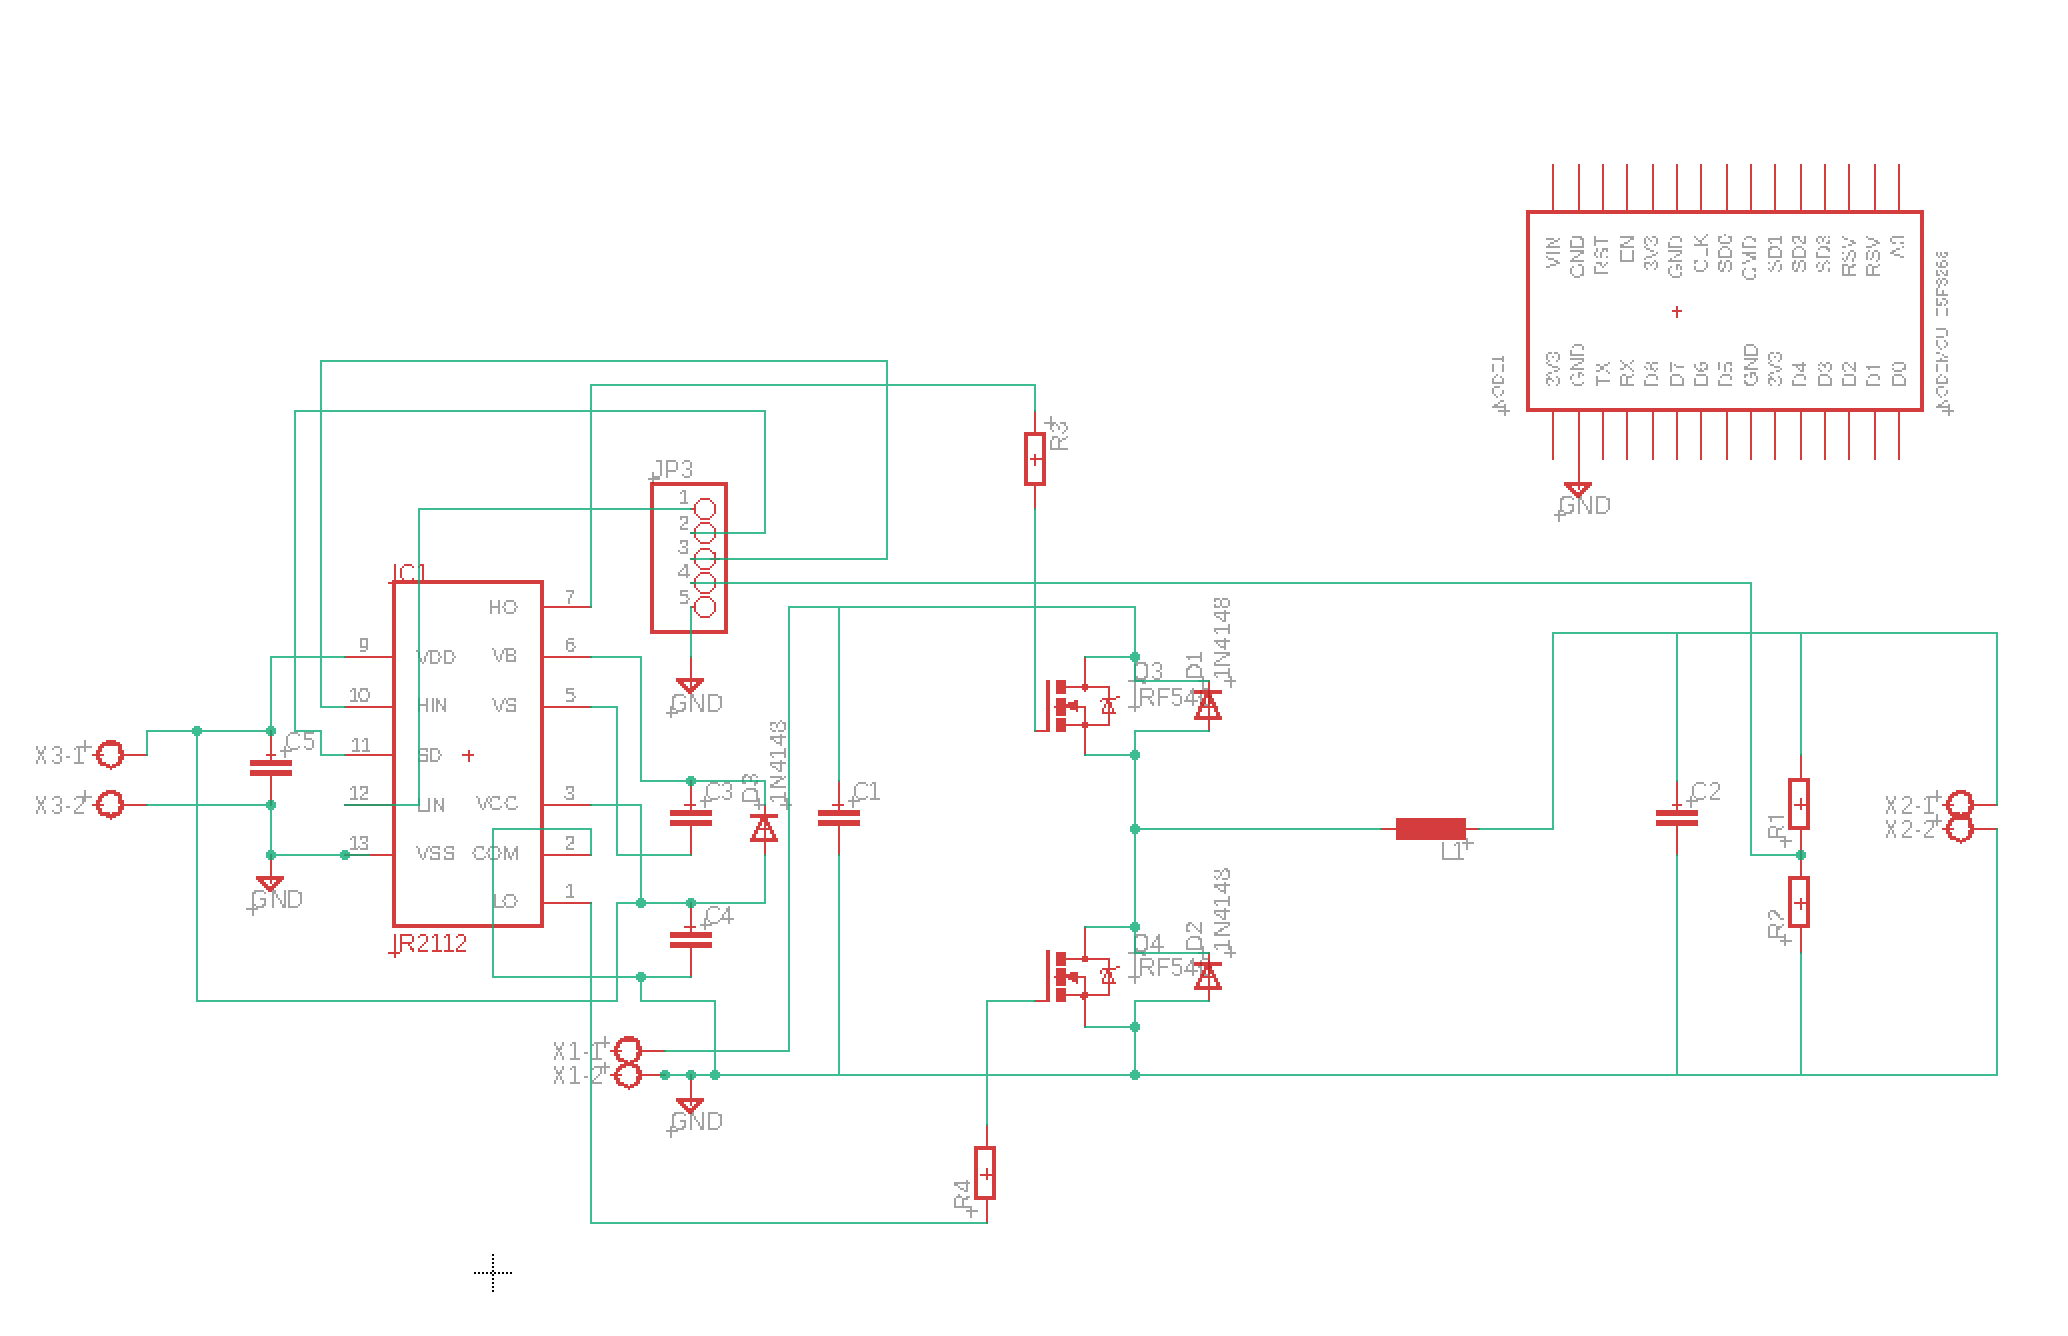
\includegraphics[width=\textwidth]{SCH_layout.png}
        \caption{Schemat ideowy Eagle}
        \label{fig:sch_eagle}
    \end{subfigure}
    \hfill
    \begin{subfigure}[b]{0.48\textwidth}
        \centering
        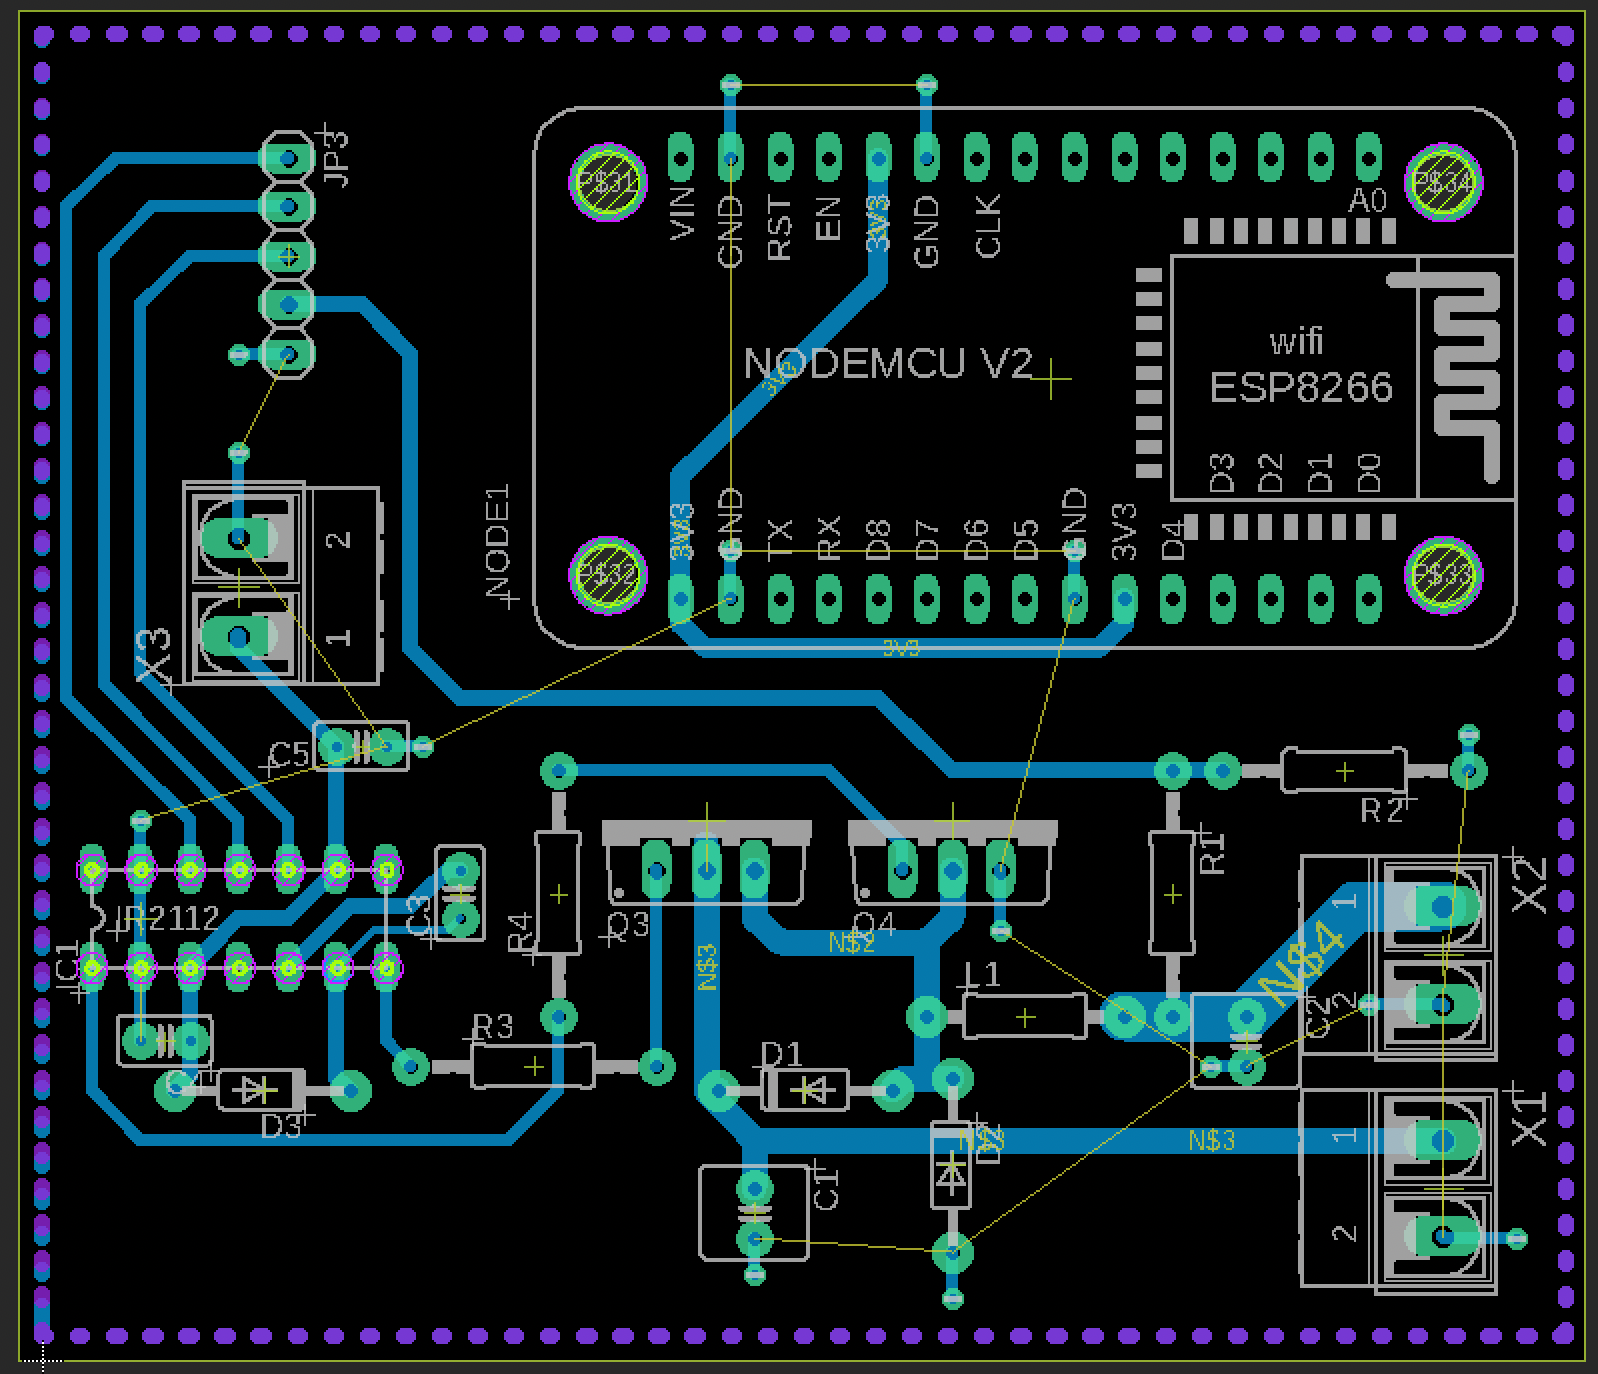
\includegraphics[width=\textwidth]{PCB_layout.png}
        \caption{Layout PCB}
        \label{fig:pcb_layout}
    \end{subfigure}
    \caption{Projekt PCB w programie EAGLE}
    \label{fig:eagle}
\end{figure}

\noindent Główne założenia projektowe płytki:
\begin{itemize}
    \item Ścieżki toru mocy ($V_{in}$, $V_{SW}$, $V_{out}$) o zwiększonej szerokości
          minimalizującej rezystancję i nagrzewanie,
    \item Kondensatory odsprzęgające przy zasilaniu IR2112 umieszczone jak najbliżej
          układu,
    \item Moduł NodeMCU umieszczony z dala od toru mocy w celu redukcji zakłóceń EMI
          wpływających na tor RF anteny,
    \item Złącza X1 (wejście), X2 (wyjście) i X3 (zasilanie logiki) na krawędziach płytki.
\end{itemize}

%% ============================================================
%% 4. SYMULACJA LTSPICE
%% ============================================================
\section{Symulacja w LTSpice}

\subsection{Parametry symulacji}

Symulację przeprowadzono z następującymi parametrami:

\begin{table}[H]
    \centering
    \caption{Parametry symulacji LTSpice}
    \label{tab:sim_params}
    \begin{tabular}{ll}
        \toprule
        \textbf{Parametr} & \textbf{Wartość} \\
        \midrule
        Napięcie wejściowe $V_{in}$       & \SI{100}{V} \\
        Częstotliwość PWM $f_{sw}$        & \SI{50}{kHz} \\
        Indukcyjność $L_1$                & \SI{100}{\micro H} \\
        Pojemność $C_1$                   & \SI{100}{\micro F} \\
        Rezystancja obciążenia $R_{load}$ & \SI{10}{\ohm} \\
        Czas symulacji                    & \SI{2}{ms} \\
        Krok symulacji                    & \SI{1}{\micro s} \\
        Sweep wypełnienia $D$             & 0,3 -- 0,7 (krok 0,1) \\
        \bottomrule
    \end{tabular}
\end{table}

\subsection{Wyniki symulacji}

\begin{figure}[H]
    \centering
    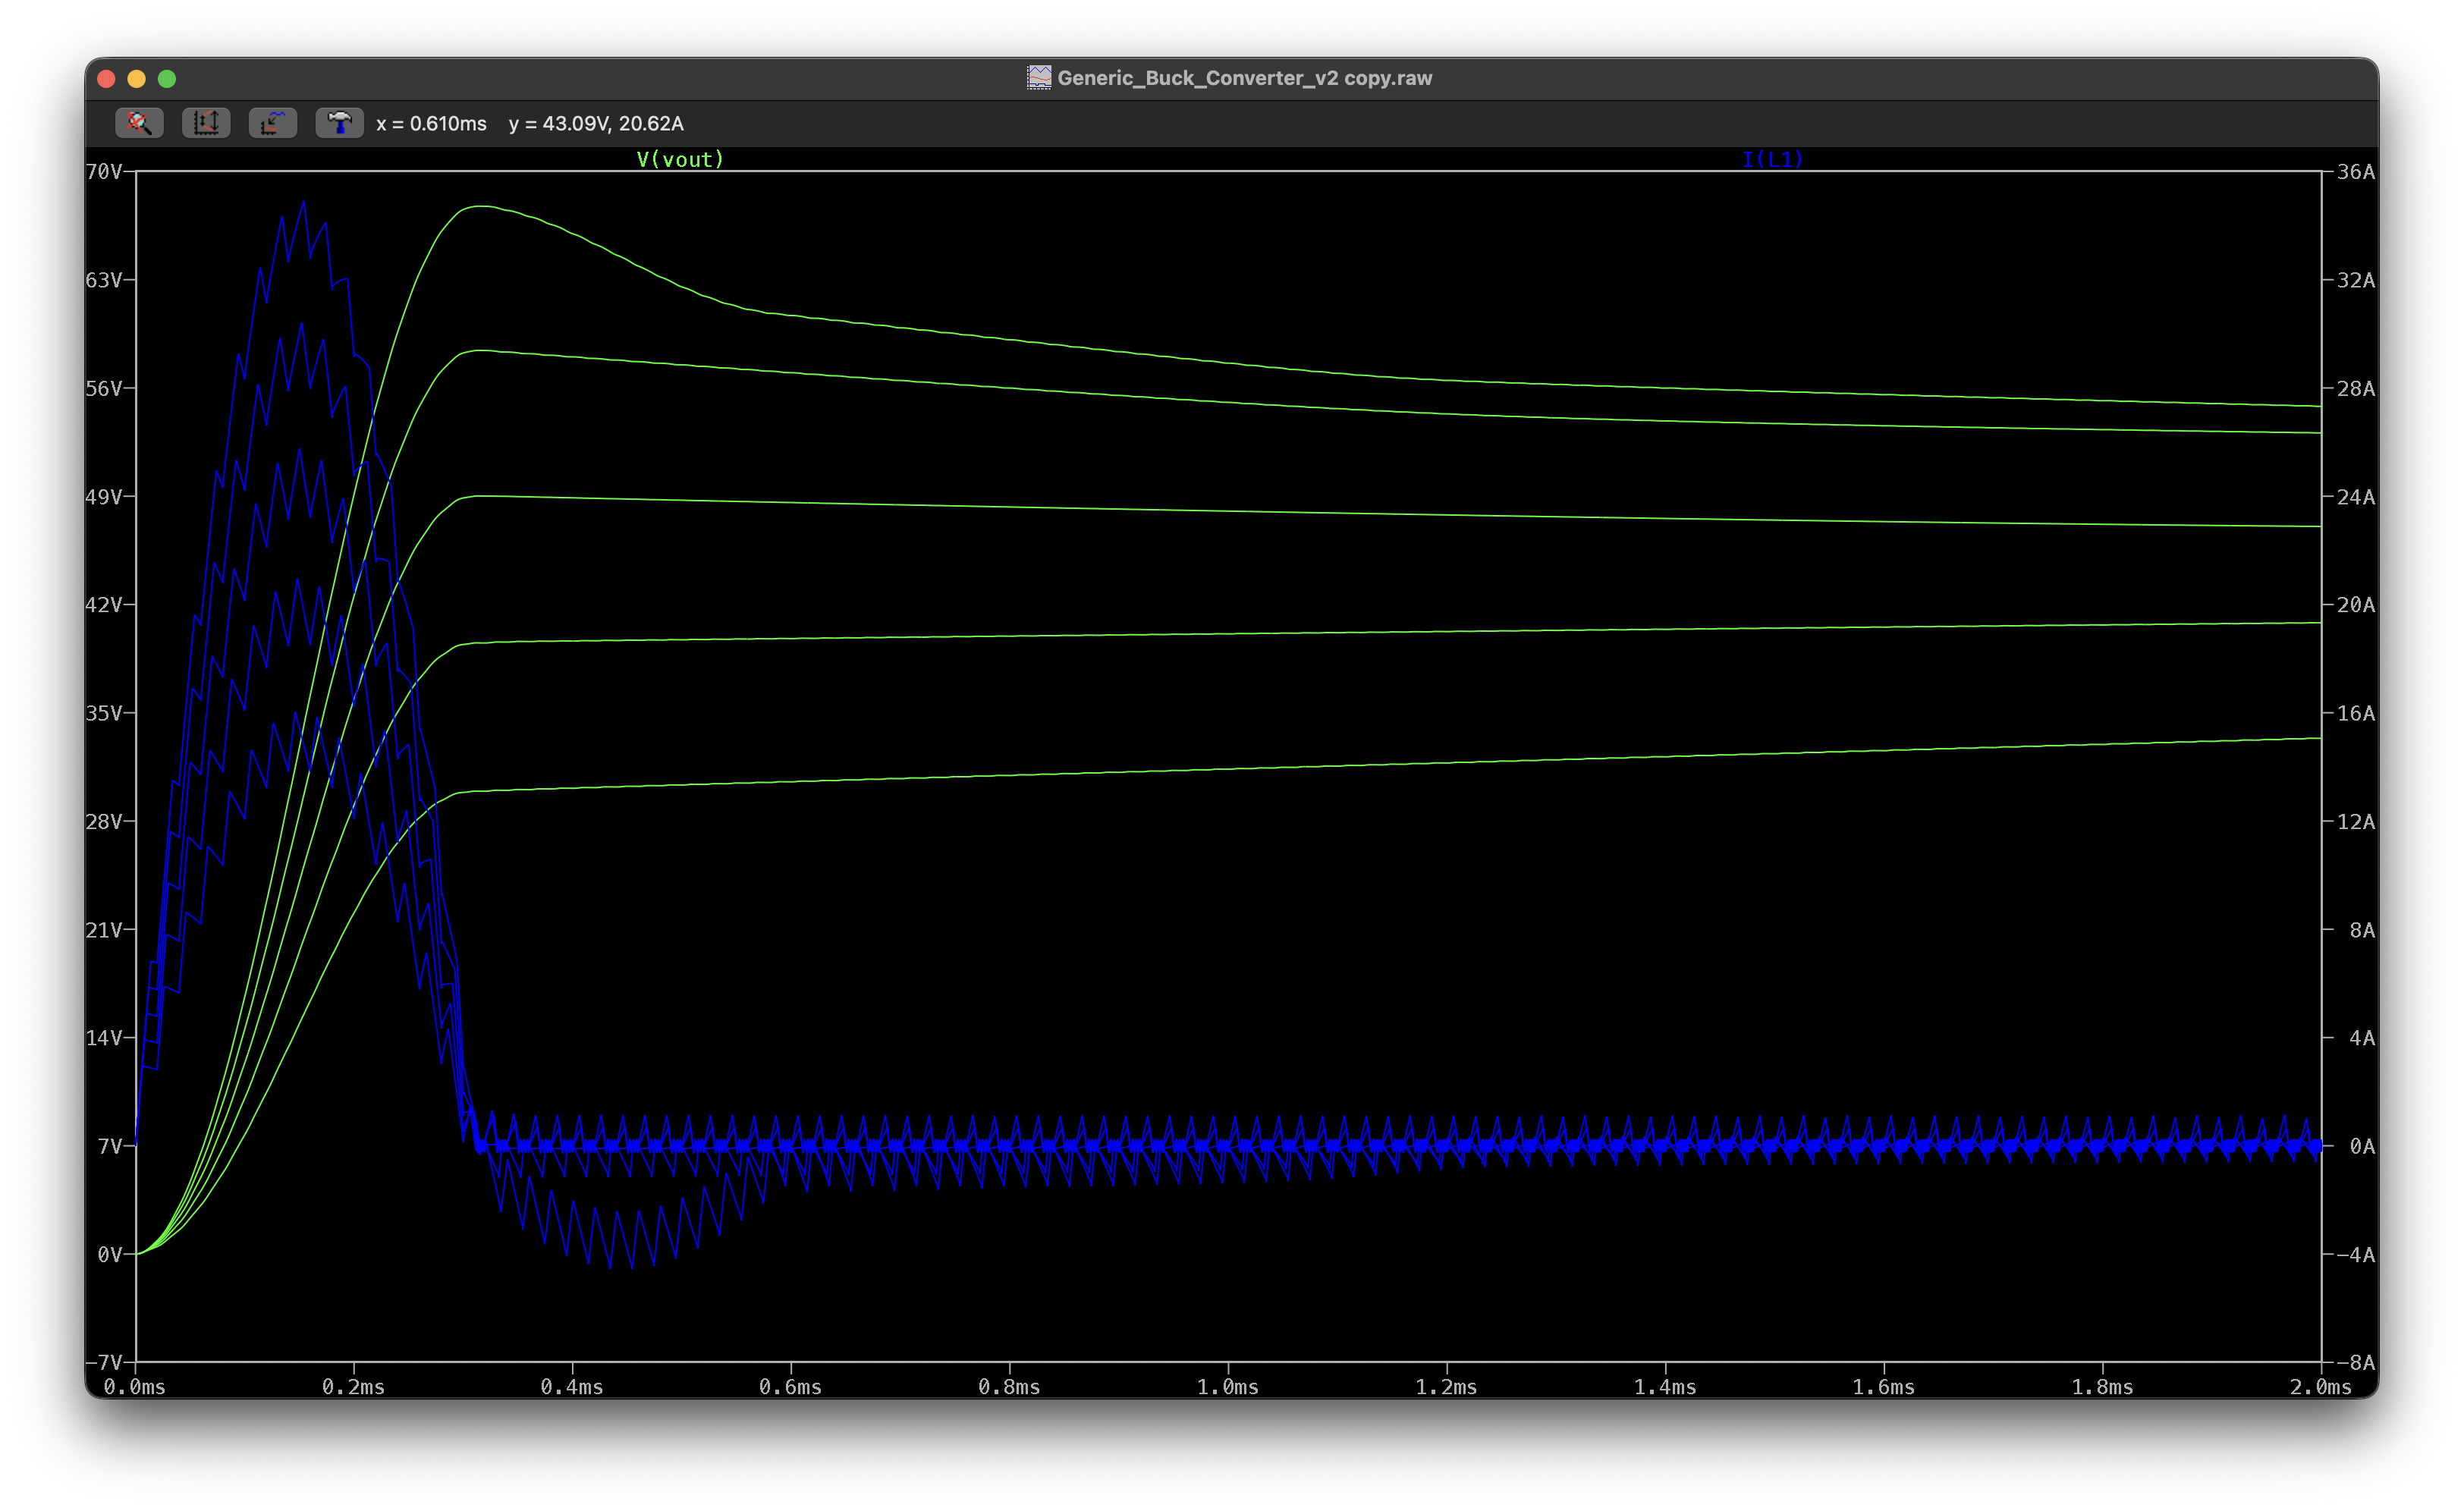
\includegraphics[width=0.95\textwidth]{Vout_I(L).png}
    \caption{Przebiegi $V_{out}$ (zielony) i $I_{L1}$ (niebieski) dla wypełnienia
             $D = 0{,}3 \div 0{,}7$}
    \label{fig:sim_results}
\end{figure}

\subsubsection{Napięcie wyjściowe}

Zmierzone napięcia wyjściowe w stanie ustalonym porównano z wartościami teoretycznymi
wynikającymi ze wzoru~\eqref{eq:buck_basic}:

\begin{table}[H]
    \centering
    \caption{Porównanie napięć wyjściowych -- teoria vs symulacja}
    \label{tab:vout}
    \begin{tabular}{cccc}
        \toprule
        \textbf{Duty} $D$ & $V_{out}$ teoretyczne & $V_{out}$ symulacja & \textbf{Błąd} \\
        \midrule
        0,3 & \SI{30}{V} & \SI{\approx 32}{V} & $+6{,}7\%$ \\
        0,4 & \SI{40}{V} & \SI{\approx 40}{V} & $\approx 0\%$ \\
        0,5 & \SI{50}{V} & \SI{\approx 47}{V} & $-6{,}0\%$ \\
        0,6 & \SI{60}{V} & \SI{\approx 57}{V} & $-5{,}0\%$ \\
        0,7 & \SI{70}{V} & \SI{\approx 65}{V} & $-7{,}1\%$ \\
        \bottomrule
    \end{tabular}
\end{table}

Odchylenia od wartości idealnych wynikają ze spadków napięcia na rezystancji
przewodzenia $R_{DS(on)}$ tranzystorów IRFP4668 oraz na indukcyjności pasożytniczej ESR cewki.

\subsubsection{Prąd cewki i tryb pracy DCM}

Z przebiegu $I_{L1}$ (rys.~\ref{fig:sim_results}) wynika, że po fazie rozruchu
przetwornica pracuje w trybie DCM -- prąd cewki spada do zera przed kolejnym
cyklem przełączania. Graniczna indukcyjność dla trybu CCM według wzoru~\eqref{eq:lmin}:

\begin{equation}
    L_{min} = \frac{(1-0{,}5) \cdot 10}{2 \cdot 50\,000} = \SI{50}{\micro H}
\end{equation}

Przy $L_1 = \SI{100}{\micro H} > L_{min}$ przetwornica powinna pracować w trybie CCM,
jednak przy $R_{load} = \SI{10}{\ohm}$ prąd średni cewki jest mały (~\SI{5}{A}),
co przy uwzględnieniu rzeczywistych parametrów tranzystorów skutkuje wejściem w DCM.

\subsubsection{Prąd rozruchowy}

Podczas rozruchu (0--\SI{0,4}{ms}) obserwowano prąd cewki sięgający \SI{32}{A}
oraz przepięcie $V_{out}$ powyżej wartości ustalonej. Jest to typowe zjawisko dla
przetwornicy pracującej w pętli otwartej bez regulatora PI/PID.
W rzeczywistym układzie regulator ogranicza prąd rozruchowy przez stopniowe
zwiększanie wypełnienia (\textit{soft-start}).

%% ============================================================
%% 5. WNIOSKI
%% ============================================================
\section{Wnioski}

\begin{enumerate}
    \item Symulacja LTSpice potwierdziła poprawność zasady działania synchronicznej
          przetwornicy buck -- napięcie wyjściowe jest proporcjonalne do wypełnienia PWM
          zgodnie z zależnością $V_{out} = D \cdot V_{in}$.

    \item Odchylenia od wartości idealnych (do $\approx 7\%$) wynikają ze strat
          przewodzenia tranzystorów i elementów pasożytniczych, co jest zgodne
          z oczekiwaniami dla modeli realistycznych.

    \item Przetwornica pracuje w trybie DCM przy zastosowanym obciążeniu \SI{10}{\ohm}.
          Przejście do trybu CCM można uzyskać przez zmniejszenie indukcyjności $L_1$
          lub zwiększenie prądu obciążenia.

    \item Duży prąd rozruchowy (~\SI{32}{A}) wskazuje na konieczność implementacji
          funkcji \textit{soft-start} w rzeczywistym układzie sterowania.

    \item Projekt PCB uwzględnia wymagania EMI przez separację toru mocy od toru
          sygnałowego ESP8266 z anteną RF. Strome zbocza $V_{SW}$ przy
          $f_{sw} = \SI{50}{kHz}$ generują zakłócenia w paśmie \SIrange{20}{100}{MHz},
          co wymaga starannego projektu PCB i opcjonalnie filtrów EMI.
\end{enumerate}

\end{document}
